% arara: pdflatex
% !arara: biber
% !arara: pdflatex
% How to run: 
% 1) pdflatex "filename".tex
% 2) biber "filename"
% 3) pdflatex "filename".tex
% 4) pdflatex "filename".tex


\documentclass[x11names]{article}
\usepackage{verbatim}
\usepackage{listings}
\usepackage{graphicx}
\usepackage{a4wide}
\usepackage{color}
\usepackage{amsmath}
\usepackage{amssymb}
\usepackage[dvips]{epsfig}
\usepackage[T1]{fontenc}
% \usepackage{cite} % [2,3,4] --> [2--4]
\usepackage{shadow}
\usepackage{hyperref}
\usepackage{physics}
\usepackage{url}
\usepackage{tikz}
\usepackage{subcaption}
\usepackage[utf8]{inputenc}
\usepackage{booktabs} % Allows the use of \toprule, \midrule and \bottomrule in tables
\usepackage[font={small,it}]{caption}
\usepackage[margin=0.7in]{geometry} %Sets the margins in the document
\usepackage{siunitx}    %Allows use of SI units macros

%Defines calculator way to write powers of ten
\sisetup{output-exponent-marker=\textsc{e}}
\renewcommand{\va}{\vec}


% Change numbering and some commands
% \renewcommand\thesection{Exercise \Roman{section}}
% \renewcommand\thesubsection{\Roman{section}.\alph{subsection}}

%% references
\usepackage[style=authoryear,
            bibstyle=authoryear,
            backend=biber,
            % refsection=chapter,
            maxbibnames=99,
            maxnames=2,
            firstinits=true,
            uniquename=init,
            natbib=true,
            dashed=false]{biblatex}

\addbibresource{bibliography.bib}
% \addbibresource{top.bib}

% \bibliography{bibliography}
% \bibliography{top}


\usepackage[capitalize]{cleveref}

\setcounter{tocdepth}{2}

\lstset{language=c++}
\lstset{alsolanguage=[90]Fortran}
\lstset{basicstyle=\small}
\lstset{backgroundcolor=\color{white}}
\lstset{frame=single}
\lstset{stringstyle=\ttfamily}
\lstset{keywordstyle=\color{red}\bfseries}
\lstset{commentstyle=\itshape\color{blue}}
\lstset{showspaces=false}
\lstset{showstringspaces=false}
\lstset{showtabs=false}
\lstset{breaklines}


\definecolor{keywords}{RGB}{255,0,90}
      \definecolor{comments}{RGB}{0,0,113}
      \definecolor{red}{RGB}{160,0,0}
      \definecolor{green}{RGB}{0,150,0}
       
      \lstset{language=Python, 
              basicstyle=\ttfamily\small, 
              keywordstyle=\color{keywords},
              commentstyle=\color{comments},
              stringstyle=\color{red},
              showstringspaces=false,
              identifierstyle=\color{green}
              }



\title{ Exercise 3 \\ Sommerjobb Numeriske Plasmaoppgaver }
\author{Gullik Vetvik Killie
		}


%%%%%%%%%%%%%%%%%%%%%%%%%%%%%%%%%%%%%%%%%%%%%%%%%%%%%%%%%%%%%%%%%%%%%%%%%%%%%%%%%%%%
% Actual text starts here
%%%%%%%%%%%%%%%%%%%%%%%%%%%%%%%%%%%%%%%%%%%%%%%%%%%%%%%%%%%%%%%%%%%%%%%%%%%%%%%%%%%%
\begin{document}


\maketitle

\section{}

\subsection{Theory}

In this text we will simulate an oxygen ion, \(O^+\) and an electron, \(e\) in the dipole field of the earth. We will use Euler's method to get the discretization of the position and work in Cartesian coordinates. From the simulation we will plot the trajectory the particles will follow, and also examine how the kinetic energy of the the particles evolve as they move along the magnetic field lines.

An approximation of Earth's dipole magnetic field is
\begin{align}
      \va{B}(\va{r}) &= \frac{\mu_0}{4\pi}\left(\frac{3\va{r}\left( \va{m} \cdot \va{r}\right)}{r^5} - \frac{\va{m}}{r^3}\right)
\end{align}
where \( \va{r} \), \(\mu_0\) and \(\va{m}\) is the position, vacuum permeability and magnetic moment respectively.

The equation of motion for a charged particle is then

\begin{align}
      \pdv{\va{v}}{t} &= \frac{q}{m}\left( \va{v} \cross \va{B}(\va{r}) \right)
      \qquad{\text{and}} \qquad
      \pdv{\va{r}}{t} = \va{v}  \label{eq:EoM}
\end{align}

Using Euler's method to dicretize it we arrive at the following two equations

\begin{align}
      \va{v}(t+h) &= \va{v}(t) + h\frac{q}{b} \left( \va{v}(t) \cross \va{B}(\va{r}(t)) \right)
      \\
      \va{r}(t+h) &= \va{r}(t) + h \va{v}(t)
\end{align}

Then we use the same algorithm as in the earlier exercises to move forward in time

 \begin{enumerate}
            \item Declare variables necessary variables.
            \item Set initial conditions
            \item For-loop over timesteps. 
                  \begin{itemize}
                        \item Update \( \va{v}(t+h) \) and \( \va{r}( t+h ) \).
                  \end{itemize}
            \item Plot and analyze results
\end{enumerate}

  \subsubsection{Runge Kutta 4}
    Let the phase-space vector \(\va{y}(t)\) represent the position and velocity of the particle, then let us use the following definitions.

    \begin{align}
      \pdv{\va{y}(t)}{t} &= \va{f}(t,\va{y})
      \\
      \va{y}(t) &= \int \va{f}(t,\va{y})\differential{t}
      \\
      \va{y}_{i+1} &= \va{y}_i + \int^{t_{i+1}}_{t_i} \va{f}(t,\va{y})\differential{t} \label{eq:next_y}
      \intertext{Using Simpson's approximation for the integral we arrive at}
      \int^{t_{i+1}}_{t_i} \va{f}(t,\va{y})\differential{t} &\approx \frac{h}{6}\left[ \va{f}(t_i, \va{y}_i) + 4 \va{f}(t_{i + 1/2} , \va{y}_{i + 1/2}) + \va{f}(t_{i + 1} , \va{y}_{i + 1}) \right]
      \intertext{To get the fourth order Runge Kutta, we divide the middle step in two.}
      \int^{t_{i+1}}_{t_i} \va{f}(t,\va{y})\differential{t} &\approx \frac{h}{6}\left[ \va{f}(t_i, \va{y}_i) + 2 \va{f}(t_{i + 1/2} , \va{y}_{i + 1/2})  + 2 \va{f}(t_{i + 1/2} , \va{y}_{i + 1/2}) + \va{f}(t_{i + 1} , \va{y}_{i + 1}) \right] \label{eq:RK4} 
    \end{align}
    \noindent Since we don't know the values of \( \va{y}_{i + 1/2}\) and \( \va{y}_{i + 1} \) so we approximate them by Euler's method

    \begin{enumerate}
      \item We know everything to compute the first step 
              \[ k_1 = h\va{f}(t_i, \va{y}_i) \]
      \item Now we use the Euler method to get \( y_{i + 1/2} \approx y_i + \frac{h}{2} \va{f}( t_i, y_i ) = y_i + \frac{k_1}{2} \) 
      \[ k_2 = h\va{f}\left(t_i + \frac{h}{2}, y_i + \frac{k_1}{2}\right) \]
      \item Then we use this to get a new estimate of the midpoint value
        \[ k_3 = h\va{f}\left(t_i + \frac{h}{2}, y_i + \frac{k_2}{2}\right) \]
      \item Then we use the approximation \(\va{y}_{i + 1} \approx \va{y}_i + k_3\)
        \[ k_4 = h\va{f}\left(t_i + h, y_i + k_3\right) \]
      \item Then we combine this with \cref{eq:next_y} and \cref{eq:RK4} to get
      \begin{align}
        \va{y}_{i+1} &\approx  \frac{h}{6}\left[ k_1 + 2k_2 + 2k_3 + k_4 \right]
      \end{align}
    \end{enumerate}

    Then we have an algorithm we can use to solve the equation of motion, to compute the derivatives in \(\va{f} = \pdv{y}{t}\) we use \cref{eq:EoM} 

    \begin{align}
      y = ( \va{r}, \va{v} )
      \qquad
      f = ( \va{v}, \frac{q}{m} \va{ v }\cross \va{B}(\va{r})  )
    \end{align}


\subsection{Results}
    
    \begin{figure} 
      \begin{subfigure}{0.45\textwidth}
        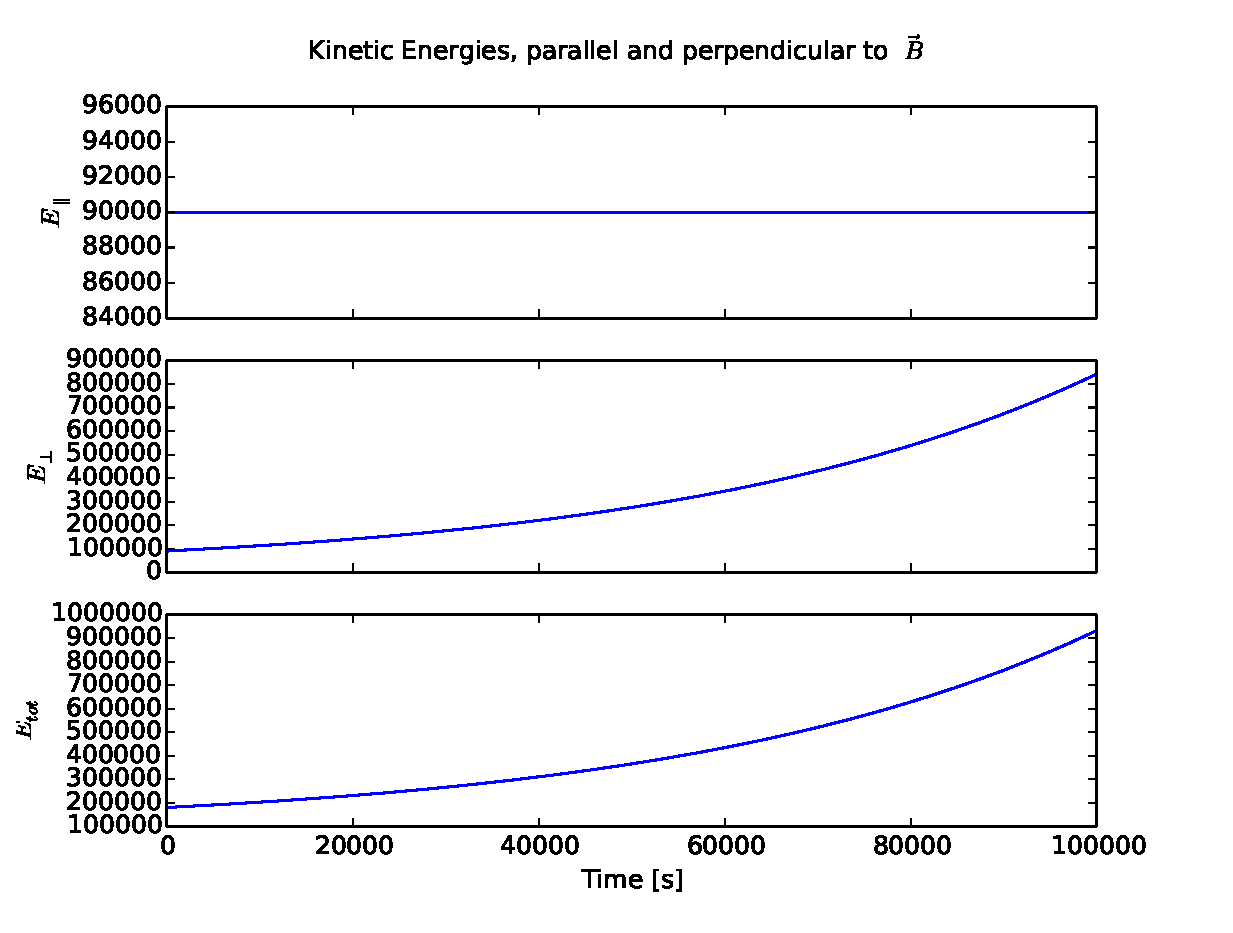
\includegraphics[width = \textwidth]{../source/figures/energyEuler_simple8-3}
      \end{subfigure}
      \begin{subfigure}{0.45\textwidth}
        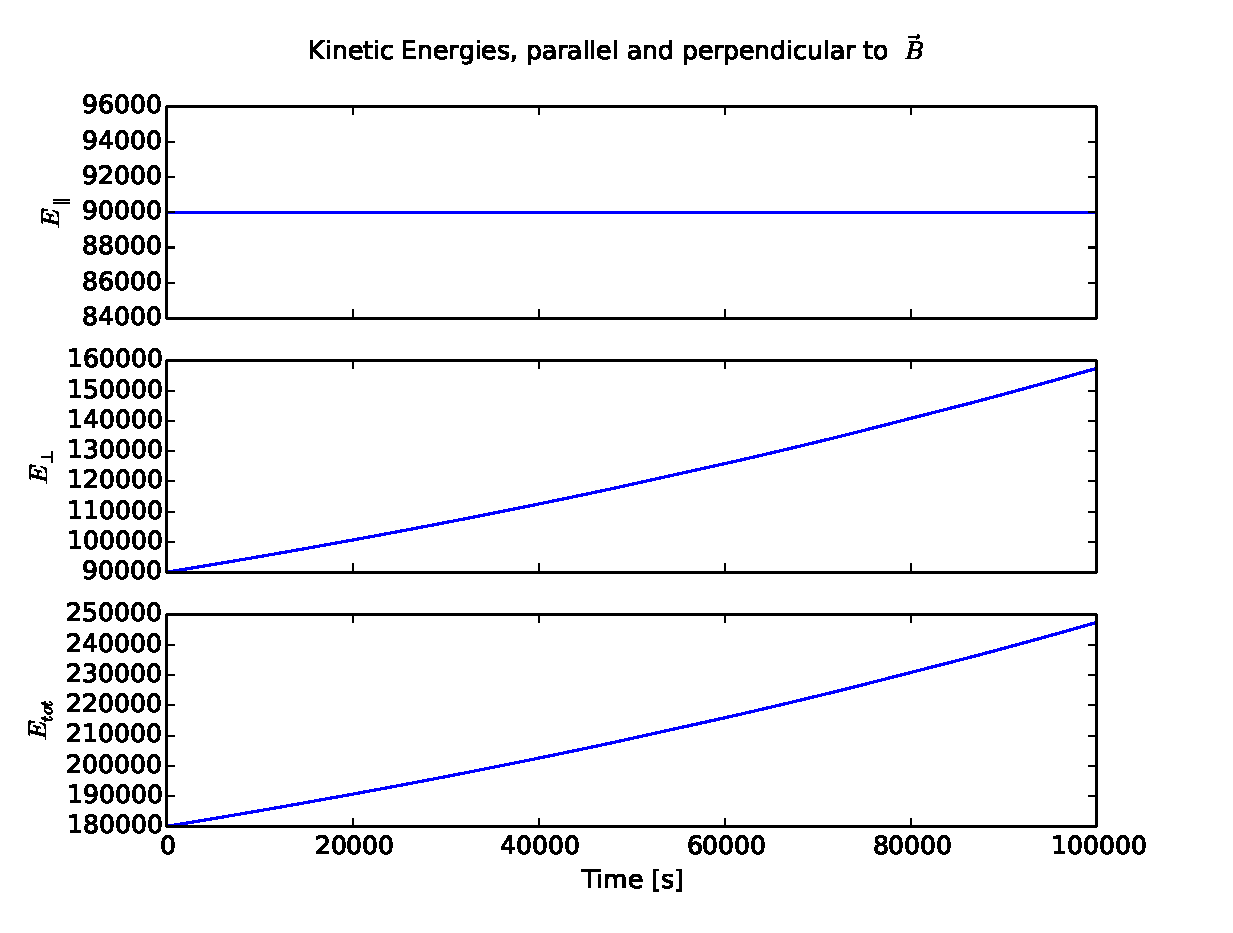
\includegraphics[width = \textwidth]{../source/figures/energyVerlet_simple8-3}
      \end{subfigure}
      \caption{The parallel, perpendicular and total energy (not multiplied with \(m/2\)) for oxygen ions in a simplified magnetic field, \(\va{B} = (0,0,0.25) nT \) z-axis running for \(10^7\) steps with \(10^{-6}\) s timesteps. Figure a) is done with Euler's method and Figure b) is done with Velocity Verlet}
      \label{fig:energy_simpleB}
    \end{figure}
    The energy results didn't really pan out well, in the \cref{fig:energy_simpleB} the perpendicular, parallel and total energy is shown for \(10^8\) steps with a timestep of \(10^{-3}\)s which should cover \(1000\) seconds, for both Euler's method and Velocity Verlet. The magnetic field is a simplified magnetic field with similar to the initial field given in the earths dipole problem \(\va{B} = (0,0,0.25) \si{\nano\tesla}\). Unfortunately there is a significant energy drift with both the methods and decreasing the timestep further makes it hard to get a long enough timeseries to look at the interesting characteristiscs happening as the particle moves in the dipole.  The Velocity Verlet has a significantly lower energy drift, but we thought it would be a symplectic integrator and conserve the energy. (Is it not symplectic when the acceleration is dependent on the velocity as well?) The energy drift is increasing with time, which would cause it to be even bigger with a longer time series.
    \\ \\

    


    We ran a simulation with a timestep of \(10^{-3}\) s for \(10^9\) steps, (\(100000 s\)), and the energy and trajectory is shown in \cref{fig:v_0_prop} for the Verlet method. As can be seen in the total energy increasing exponentially, and the trajectory deforming, the timestep is to big to accurate capture the gyrating motion. Using the Euler method it blew up completely.
    \begin{figure}[ht]
      \begin{subfigure}{0.45\textwidth}
        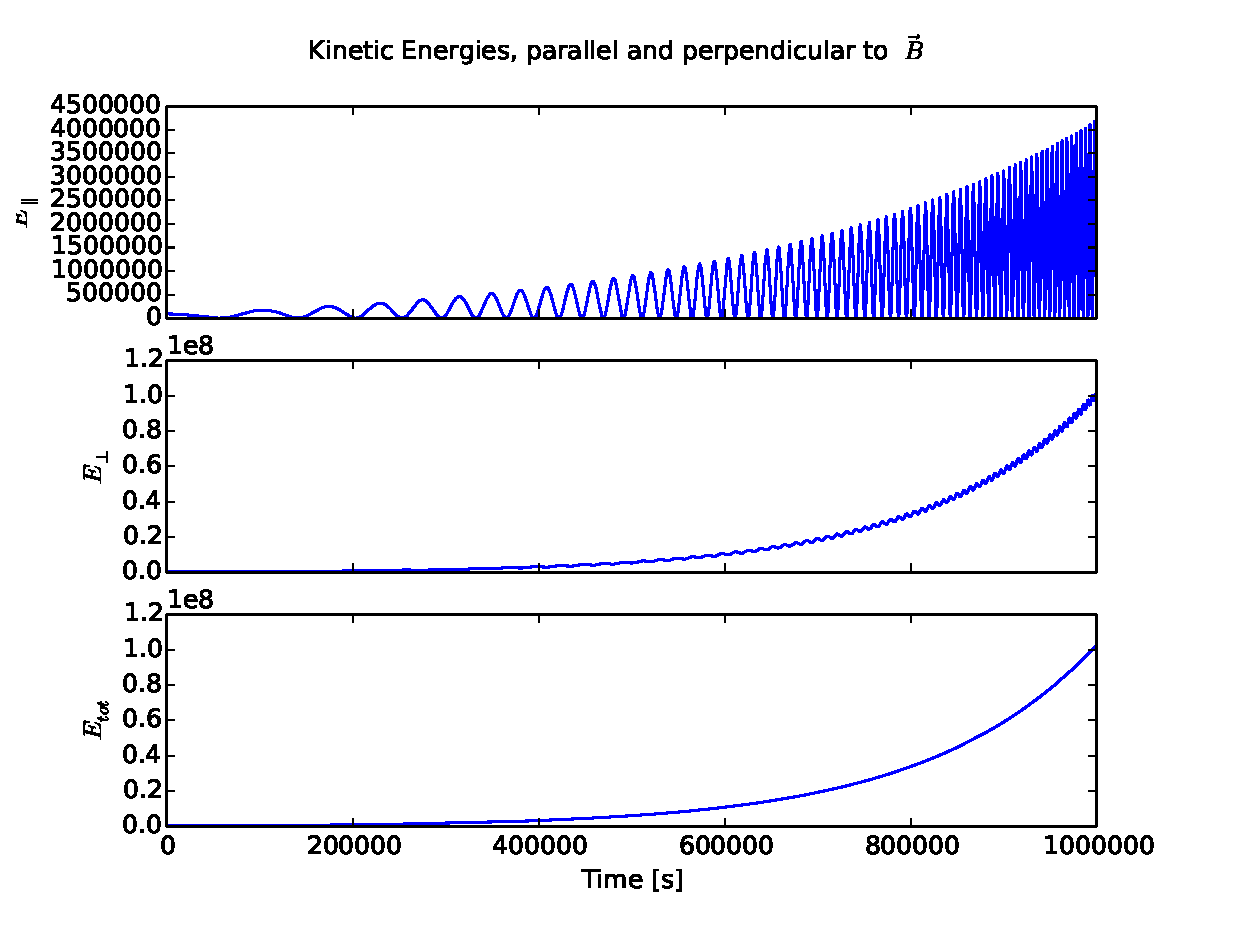
\includegraphics[width = \textwidth]{../source/figures/ion_9_3_Verletenergy}
      \end{subfigure}
      \begin{subfigure}{0.45\textwidth}
        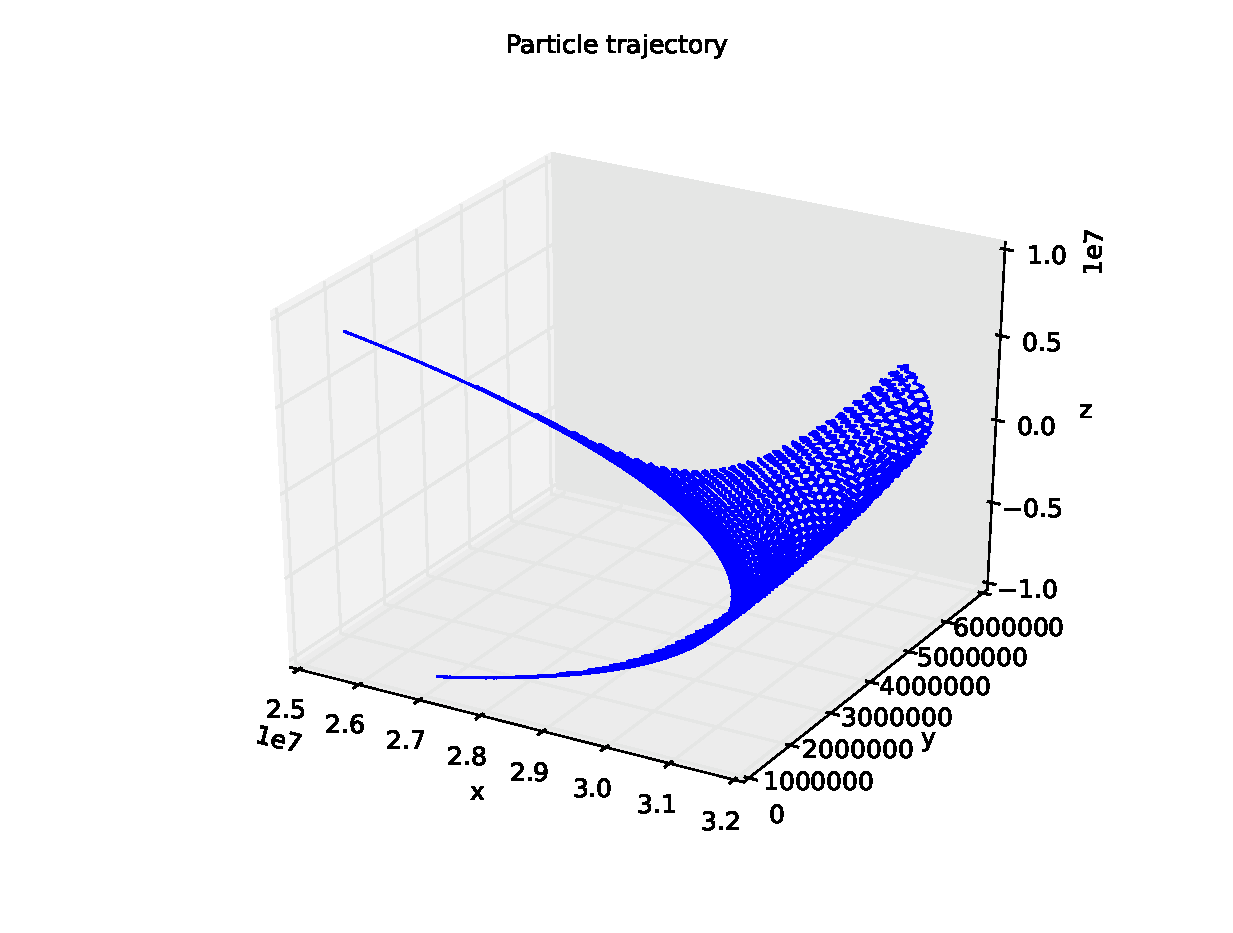
\includegraphics[width = \textwidth]{../source/figures/ion_9_3_Verlet3Dplot}
      \end{subfigure}
      \caption{The energy and trajectory for an oxygen ion for with a \(\Delta t = 10^-3\), starting at \(\va{v}_0 = (300, 0, 300) \si{ms^{-1} }\).}
      \label{fig:v_0_prop}
    \end{figure}

    By increasing the initial velocities to \(\va{v}_0 = (300000, 0, 300000) \si{\meter \per \second}\) instead of \(\va{v}_0 = (300, 0, 300) \si{\meter \per \second}\) the time needed for the effects of the dipole to show itself were shorter so we could decrease the timestep to \(10^{-5} \si{s}\) and the energy drift of the system were small enough to mostly ignore. The \cref{fig:high_vel} show an oxygen ions position, trajectory and energy during \(10^8\times 10^{-5} = 10000 \) seconds. In both the trajectory and the plot of the z-position we can clearly see that the particle is bouncing back and forth between then poles. There is also a drift in the eastward direction that can be seen most easily in the plot of the trajectory, but can also be seen as the x-coordinate is gradually decreasing and the y-coordinate is increasing.     When the parallel energy is increasing, the perpendicular energy is decreasing keeping the total energy roughly constant.


    \begin{figure}
      \begin{subfigure}{0.45\textwidth}
        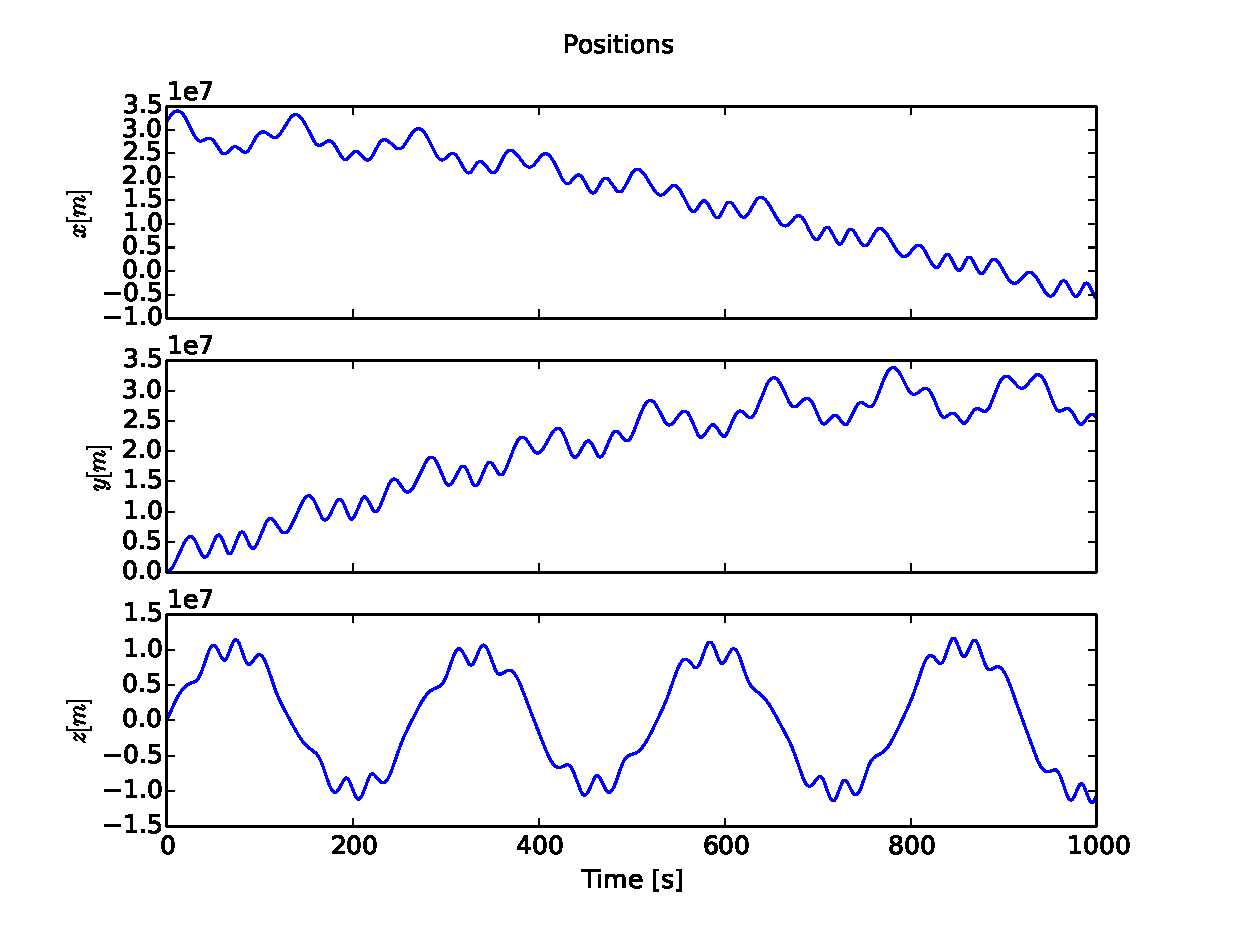
\includegraphics[width = \textwidth]{../source/figures/ion_8_5_Eulerxyz}
      \end{subfigure}
      \begin{subfigure}{0.45\textwidth}
        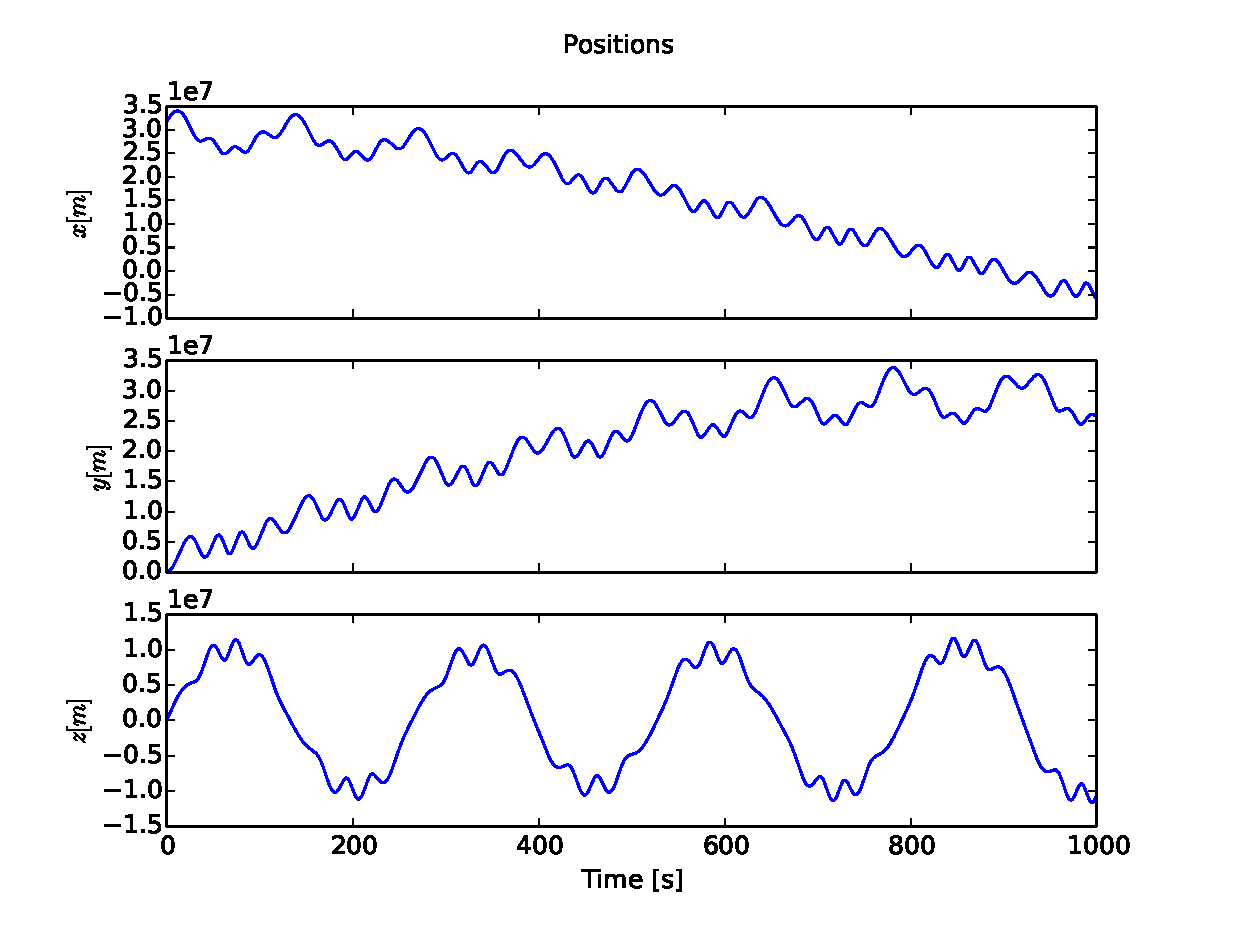
\includegraphics[width = \textwidth]{../source/figures/ion_8_5_Verletxyz}
      \end{subfigure}
      \begin{subfigure}{0.45\textwidth}
        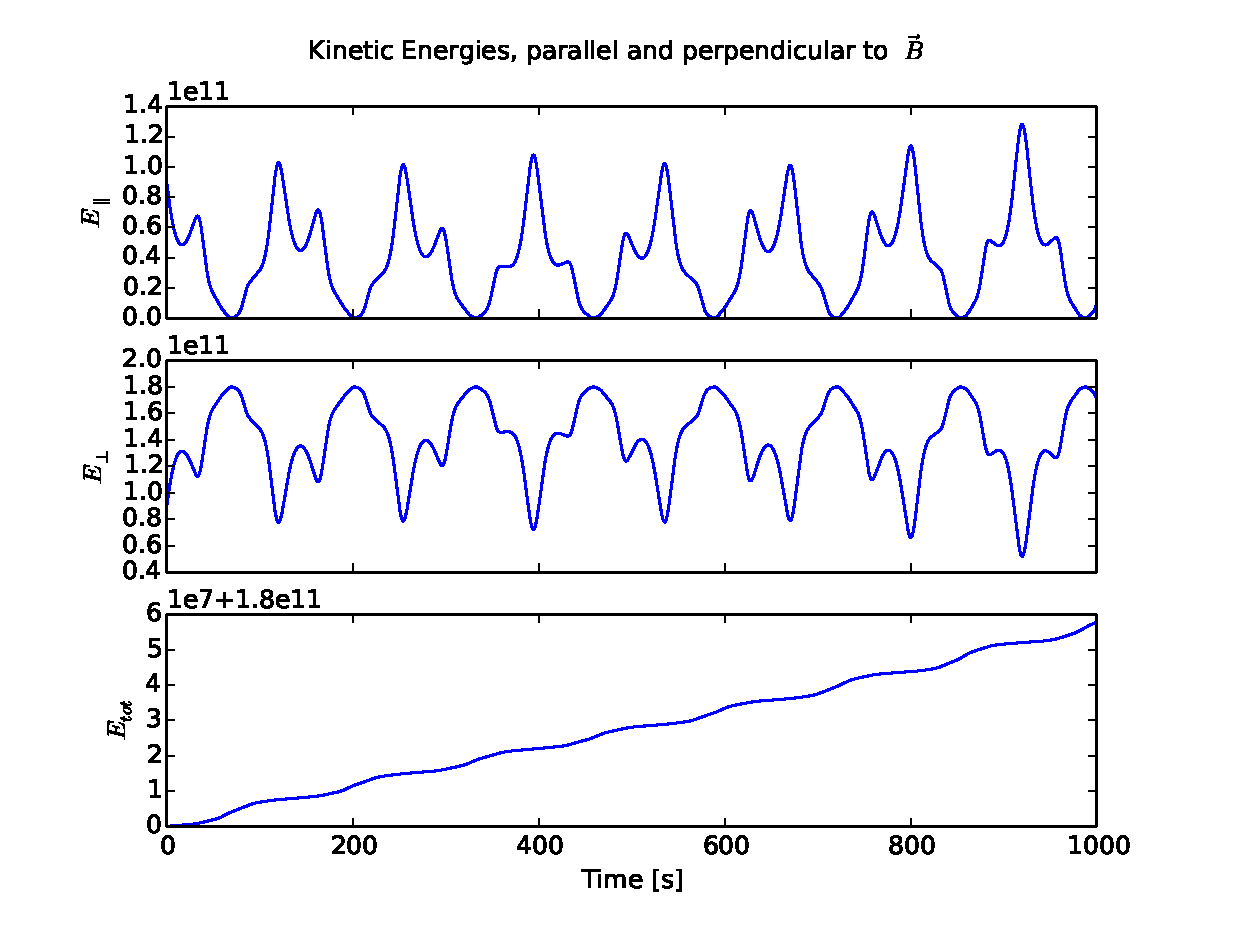
\includegraphics[width = \textwidth]{../source/figures/ion_8_5_Eulerenergy}
      \end{subfigure}
      \begin{subfigure}{0.45\textwidth}
        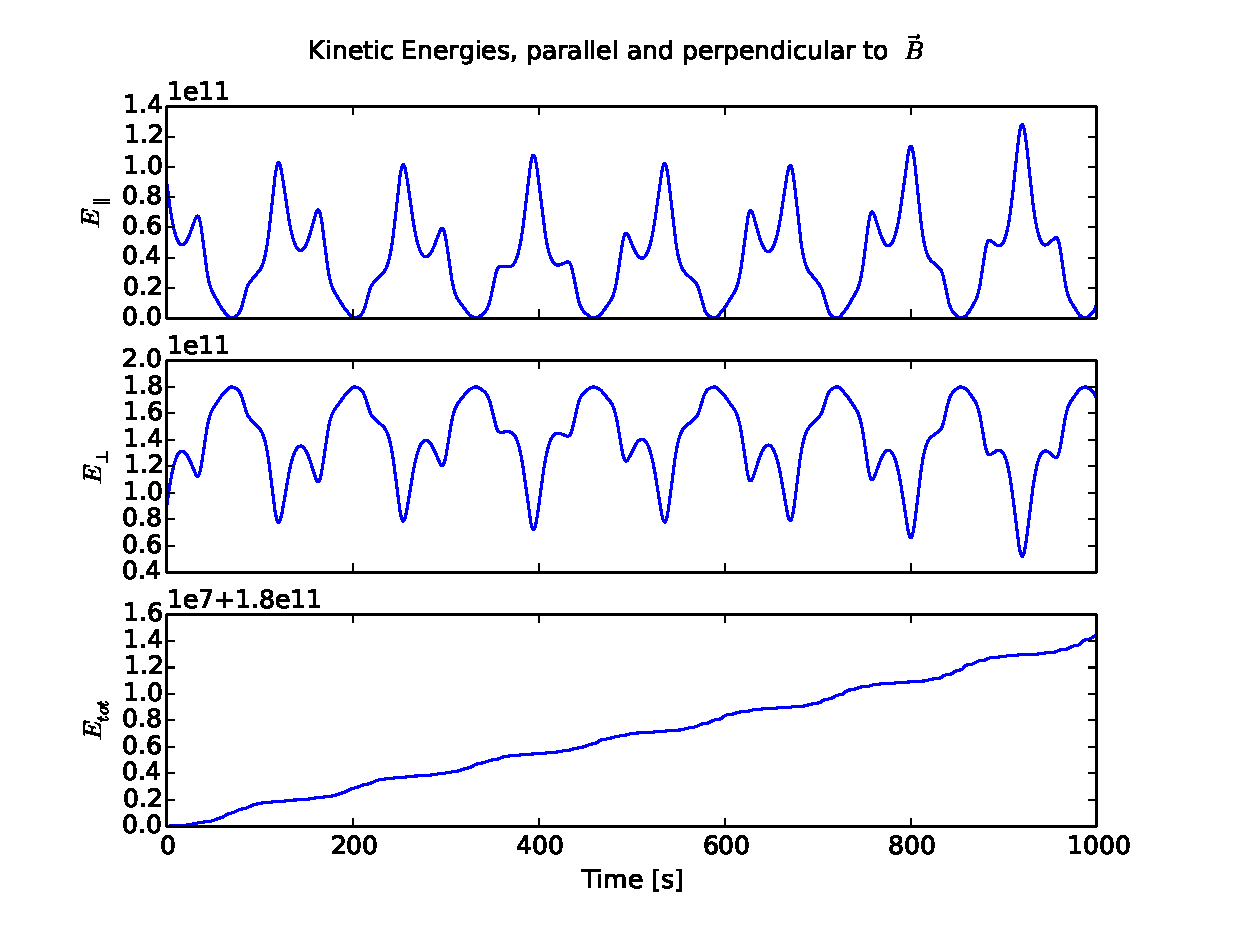
\includegraphics[width = \textwidth]{../source/figures/ion_8_5_Verletenergy}
      \end{subfigure} 
      \begin{subfigure}{0.45\textwidth}
        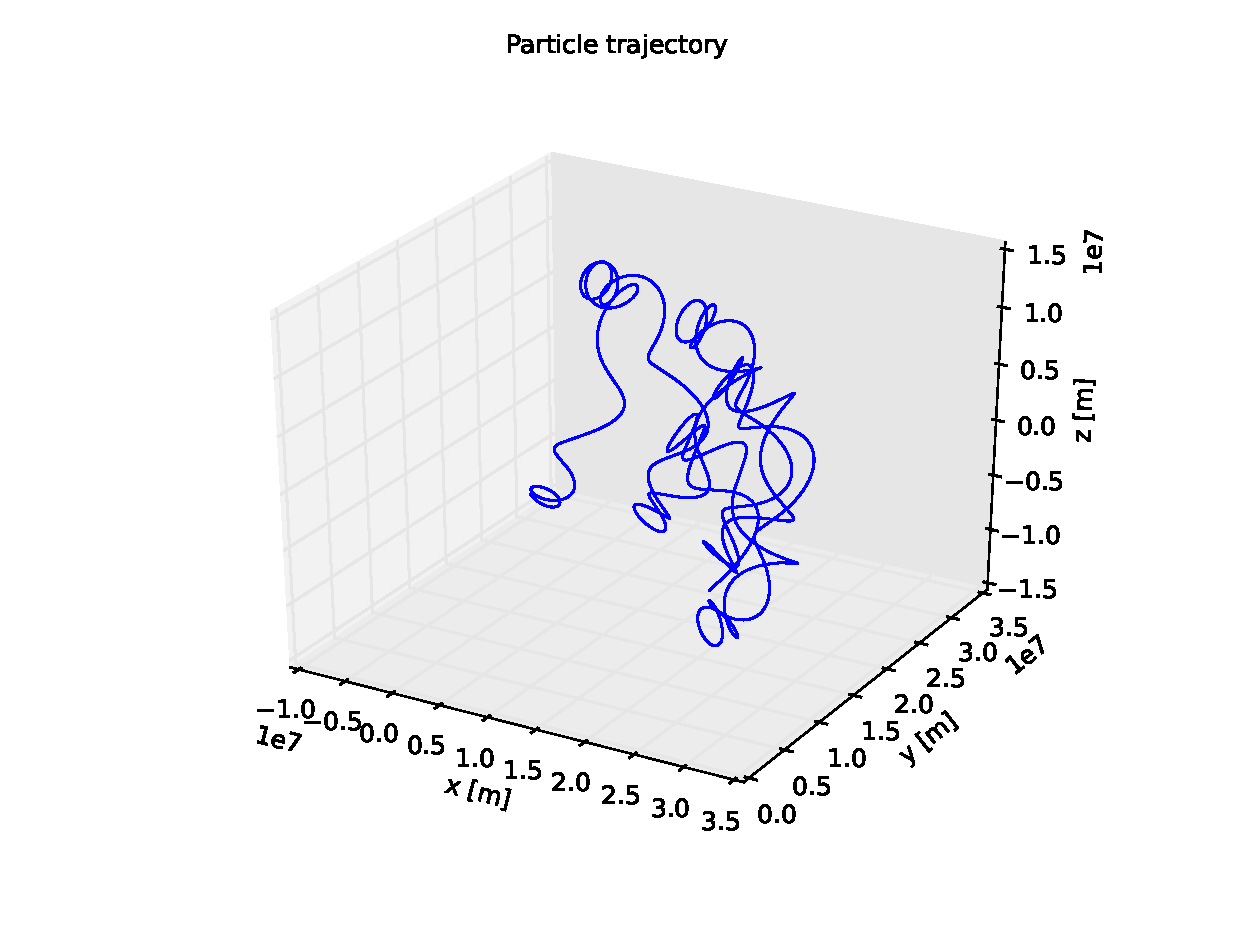
\includegraphics[width = \textwidth]{../source/figures/ion_8_5_Euler3Dplot}
      \end{subfigure}
      \begin{subfigure}{0.45\textwidth}
        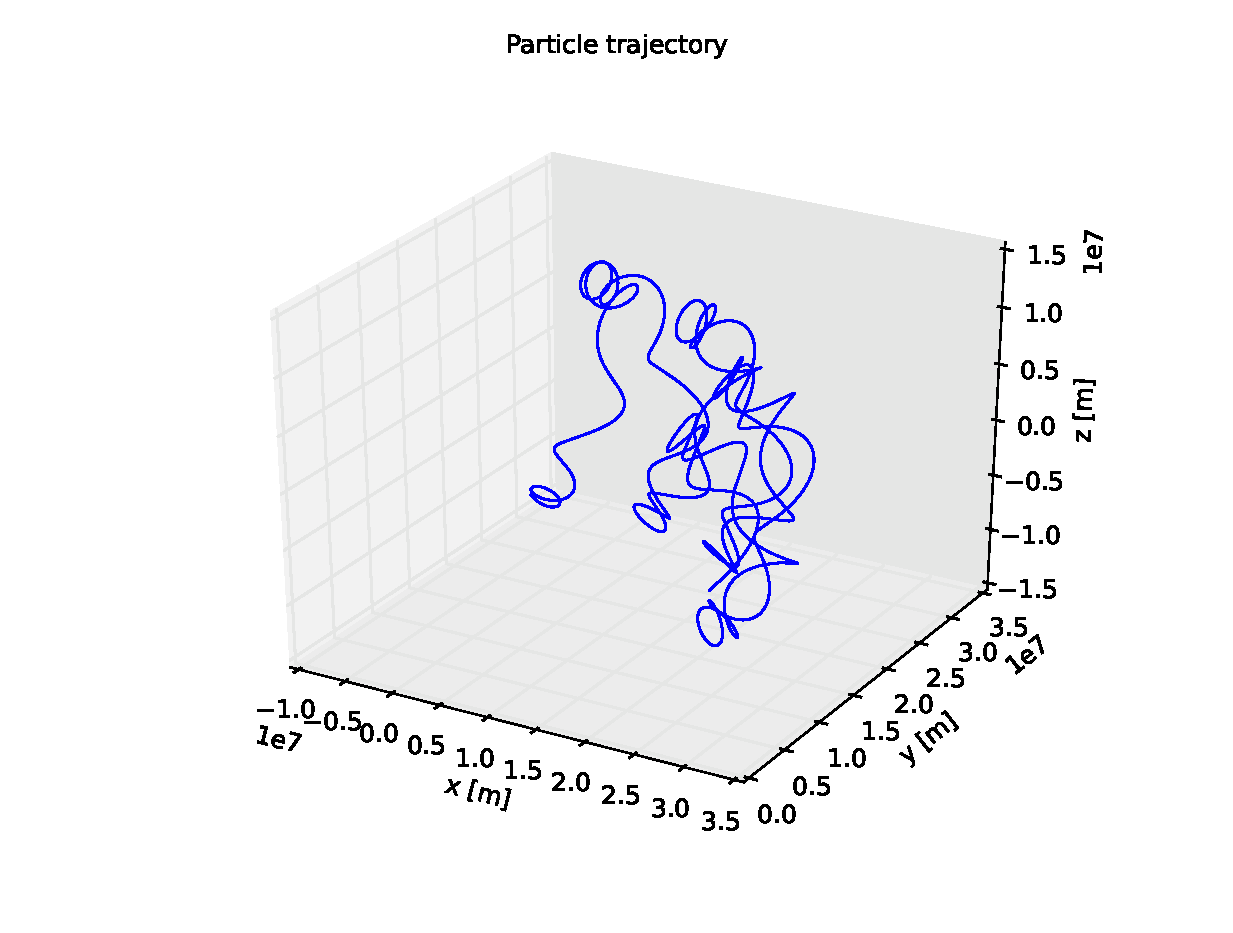
\includegraphics[width = \textwidth]{../source/figures/ion_8_5_Verlet3Dplot}
      \end{subfigure}
    \caption{This shows the positions, the energy and the trajectory of an oxygen ion trapped in earths magnetic dipole. Th figures on the left uses the Verlet Euler method, and the right figures uses the Velocity Verlet method. \(\Delta t = 10^{-5}\) and \(\va{v}_0 = (300000, 0 , 300000) m/s \).}
    \label{fig:high_vel}
    \end{figure}


    \subsubsection{Gyro period}
    Since the magnetic field is cylindrical symmetric, so let us use that and measure that as fast movements of the angle between the \(x-\) and \(y-\) coordinates. The gyration period will also change as it is dependent on \(|\va{B}|\), so the average is measured. For the run in \cref{fig:high_vel} with a high velocity an average gyration period of \( 33 \si{\second}\) was measured.

    (I didn't see any easy, robust methods to measure the gyration period)


    \subsubsection{Bounce period}
    The particle will start by moving north compared with earth following the magnetic field lines, then as the magnetic field line density increases the parallel velocity will decrease. A static magnetic field does no work on a particle so the perpendicular velocity must increase. Since it will bounce between the north and south pole, the easiest method to measure it is to note how long time it takes between each time the particle crosses equator, \(z = 0\).

    The measurements in \cref{fig:high_vel} give a rough estimate of the bounce period of \( 250 \si{\second}\)

    \subsubsection{Drift period}
    The drift period is the time a particle trapped in earths magnetic dipole field takes to drift around earth. Since we know the \(x-\) and \(y-\)coordinates we can calculate the longitude of the particles position as \( \phi = \arctan{x/y} \). Then we can roughly say that \(\Delta \phi = \arctan(\Delta x / \Delta y) \).

    The measured drift period was measured in \cref{fig:high_vel} to be \(3500 \si{\second}\).


\appendix
\section{Comments regarding the exercise}
      \begin{itemize}
            \item Parenthesis in Eq. 1 on the sheet is missing.
            \item I assume you mean the perpendicular and parallel \textit{kinetic} energy in part 2.
            \item Could it be better to plot it first, and afterwards find the energy. I think it is quite natural to plot it while working on it.
            \item I suppose we are supposed to find that the total kinetic energy is conserved (in a static magnetic field, \(\pdv{\va{B}}{t} = 0\)). Since we have to calculate so many gyrations the error caused by the Euler's method stacks up. Would it an idea to ask them to implement some almost as simple algorithm, such as as Velocity Verlet which should conserve energy better? 
            \begin{align*}
              v_i(t+\frac{h}{2}) &\approx v_i(t)  + \frac{h}{2}\frac{F_i(t)}{m} + \order{h^2} 
              \\
              x_i(t+h) &\approx x_i(t) + hv_i(t+ \frac{h} {2} ) + \order{h ^ 3}
              \\
              v_i(t+h) &\approx v_i(t+\frac{h}{2})  +  \frac{h}{2}\frac{F_i(t+ \frac{h}{2})}{m} + \order{h^2} 
            \end{align*}
            \item The stepsize per gyration needed for the Euler method was very high, to keep it somewhat well behaved after the many gyrations. With enough gyrations to mirror back and forth it needed to many steps to be contained in numpy arrays due to memory. Not recording every position fixes it though.
            \item I also implemented Velocity Verlet, and the improvement in the energy conservation is shown in the results. There was still some energy drift. Not as much an improvement as I thought there would be.
            \item I increased the velocity the particles moved in up from \(300\) to \(300 000 \si{\meter\per\second}\). Then it was much easier to get a reasonable timestep.
            \item The electron has a much faster gyration period, initial period \( \tau = \frac{m}{q|\va{B}( 5R_e, 0, 0 )|} 2\pi \sim 10^{-4}\) so then it is hard to get the particle to move enough for the magnetic field to change significantly while still keeping a small enough timestep to capture enough details on the fast gyrations.
            \item I have trouble getting much more than \(10^9 \Delta t\) in python in a reasonable time frame, on a decent laptop.
            \item Had some trouble due to some wrong numbers giving a very small \(dv\) and \(dr\) causing it to get machine-rounded away, with the right set up that problem disappeared. (my fault)
      \end{itemize}


\section{Code}
  \label{sec:code}
  \lstinputlisting{../source/dipoleField_rewritten.py}

      

\end{document}